\section{Conclusions}
This work shows that it is possible to create a knowledge graph through 
semantic relationships, also known as ontological, that exist between objects 
that are usually found in interior spaces of human occupation, such as a room. 
In fact, the characterization occurs at the moment of defining the relationship 
that two objects have to each other, following the convention: 
\texttt{object1-predicate-object2}.
% Este trabajo muestra que es posible crear un grafo de conocimiento por medio 
% de las relaciones semánticas, conocidas también como ontológicas, que existen 
% entre los objetos que usualmente se encuentran en espacios interiores de 
% ocupación humana, como una habitación. De hecho, la caracterización se da en 
% el momento de definir la relación que tiene dos objetos entre sí, siguiendo la 
% convención sugerida en \cite{Cewu}: \texttt{objeto1--predicado--objeto2}.

Thanks to Grakn it was possible to characterize objects, since through its 
high-level language it was possible to define the types of highly interconnected 
relationships between objects, since it provides a scheme that implements the 
principles of knowledge representation and reasoning.
% Gracias a Grakn fue posible caracterizar los objetos, puesto que por medio 
% de su lenguaje de alto nivel fue posible definir los tipos de relaciones 
% altamente interconectados entre los objetos, ya que proporciona un esquema que 
% implementa los principios de representación del conocimiento y razonamiento.

It is important to highlight that this is an initial work that can be extended 
depending on the needs and requirements associated with the characterization 
of objects using knowledge graphs. Its usefulness was shown with the objects 
present in a room, but the spectrum can also be extended to an entire house, 
offices, or other closed and open spaces of human occupation.
% Es importante destacar que este es un trabajo inicial que puede extenderse 
% en función de las necesidades y requerimientos asociados a la caracterización 
% de objetos mediante grafos de conocimiento. Se mostró su utilidad con los 
% objetos presentes en una habitación, pero también puede ampliarse el espectro 
% a toda una vivienda, oficinas, u otros espacios cerrados y abiertos de 
% ocupación humana. 

On the other side, since an artificial intelligence project is made up of 
several parts as needed, for the case in which knowledge graphs are involved, 
there is a phase of data acquisition and subsequently communicates with other 
systems that feed it back. This is important because the knowledge generated by 
the graph can serve as input to other models for object detection, such as 
convolutional neural networks or using YOLO systems.
% Por otro lado, dado que un proyecto de inteligencia artificial se compone de 
% varias partes según se necesite, para el caso en el que se involucran grafos 
% de conocimiento existe una fase de adquisición de datos y posteriormente se 
% comunica con otros sistemas que lo retroalimentan. Lo anterior resulta 
% importante porque el conocimiento generado por el grafo puede servir como 
% entrada a otros modelos para la detección de objetos, como las redes 
% neuronales convolucionales o utilizando sistemas YOLO.

% NEW
As mentioned, this work creates a semantic relationship of objects of an 
environment of human occupation given. This information could be useful for 
CNN models and could be added as an additional layer, called a 
``semantic layer''. This layer would work in conjunction with the CNN 
tagging phase, as shown in Figure \ref{fig:pipeline}.

\begin{figure}[H]
    \centering
    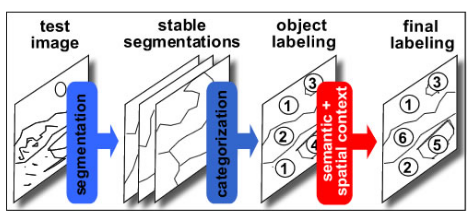
\includegraphics[width=6cm]{figures/pipeline.png}
    \caption{CNN generic pipeline model. Source \cite{Galleguillos2}}
    \label{fig:pipeline}
\end{figure}

% END NEW

Based on the results obtained, and given the usefulness of knowledge graphs 
in the characterization of objects, future work seeks to create and feed 
datasets, in JSON, XML or other formats, that contain ontological relationships 
of existing objects in a given indoor space of human occupation, such as a home, 
office and other places of rest or work. This will allow an understanding of 
the environment that surrounds users.
% Con base en los resultados obtenidos, y dada la utilidad de los grafos de 
% conocimiento en la caracterización de objetos, como trabajo futuro se busca 
% crear y alimentar datasets, en formatos JSON, XML u otro, que contengan 
% relaciones ontológicas de objetos existentes en un determinado ambiente 
% cerrado de ocupación humana, como una vivienda, oficina y otros lugares 
% de descanso o trabajo. Esto permitirá comprender el ambiente que rodea a 
% los usuarios. 

On the other side, we will seek to implement an improved version of the 
knowledge graph, in which new attributes are included, such as the 
\textit{probability of occurrence} between the relationship of two objects. 
For this approach, a previous dataset is required, from which we could count 
the relationships and then translate those data into probabilities.
% Por otro lado, se buscará implementar una versión mejorada del grafo de 
% conocimiento, en el que se incluyan nuevos atributos, como la 
% \textit{probabilidad de ocurrencia} entre la relación de dos objetos. 
% Para este enfoque se requiere de un dataset previo, del cual se puedan hacer 
% conteos de las relaciones y posteriormente traducir esos datos en 
% probabilidades.

% NEW
% b) Otro en las conclusiones, estás son débiles. Necesitas poner alguno 
% relacionado con el objetivo principal que tenías. Se logró o no el cometido 
% de caracterizar objetos a través de la relación semántica y por qué es 
% importante este tipo de análisis.

% IDEAS
% it its important because it allow us to put the right tags in the correct 
% objects, the semantic relationships gives us a lot of contextual information 
% about given objects.

%use our experience